\documentclass[journal]{IEEEtran}
\usepackage[a5paper, margin=10mm, onecolumn]{geometry}
\usepackage[cmex10]{amsmath}
\usepackage{amssymb,amsfonts,amsthm}
\usepackage{gvv-book}
\usepackage{gvv}
\usepackage{hyperref}
\usepackage{physics}

\begin{document}


\title{4.3.12}
\author{EE25BTECH11025 - Ganachari Vishwambhar}
\maketitle

\textbf{Question}:\newline
Check which of the following are solutions of the equation $x-2y=4$ and which are not\\
\begin{enumerate}
    \item $\brak{0,2}$
    \item $\brak{2,0}$
    \item $\brak{4,0}$
    \item $\brak{\sqrt{2},4\sqrt{2}}$
    \item $\brak{1,1}$
\end{enumerate}
\textbf{Solution: }\\

Given line equation can be written as:
\begin{align}
    \vec{n}^\top\vec{x}=c
\end{align}

where $\vec{n}=\myvec{1\\-2}$, $\vec{x}=\myvec{x\\y}$ and $c=4$.\\

Checking whether a point lies on the line or not by substituting given vectors in (1):
\begin{align}
    \vec{x}_1=\myvec{0\\2}, \vec{x}_2=\myvec{2\\0}, \vec{x}_3=\myvec{4\\0}, \vec{x}_4=\myvec{\sqrt{2}\\4\sqrt{2}}, \vec{x}_5=\myvec{1\\1}\\
    \vec{n}^\top\myvec{\vec{x}_1&\vec{x}_2&\vec{x}_3&\vec{x}_4&\vec{x}_5}=\myvec{c_1&c_2&c_3&c_4&c_5}\\
    \myvec{1&-2}\myvec{0&2&4&\sqrt{2}&1\\2&0&0&4\sqrt{2}&1}=\myvec{-4&2&4&-7\sqrt{2}&-1}\\
\end{align}

Conclusion:\\

The point which lies on the line is only option (3).

\begin{figure}[h!]
   \centering
   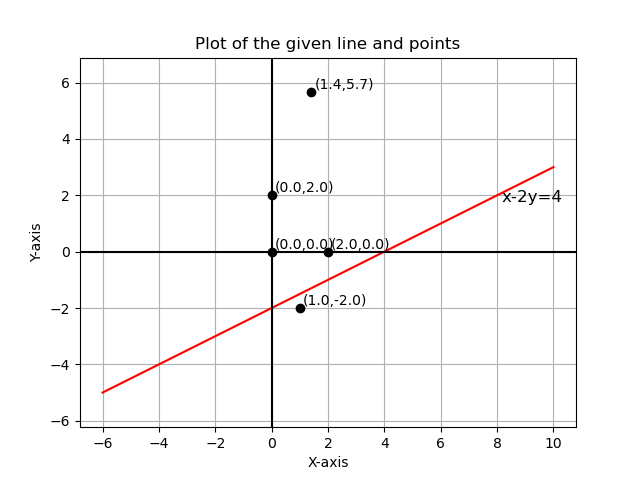
\includegraphics[width=0.7\linewidth]{figs/plot.png}
   \caption{Plot of the given line and points}
   \label{}
\end{figure}
\end{document}  
